\documentclass[tikz, border=2mm]{standalone}
\usepackage{amsmath} % Para \sqrt
\begin{document}
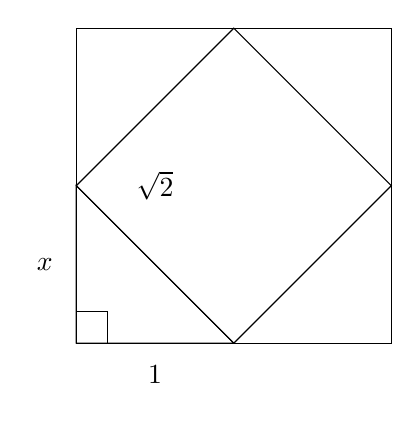
\begin{tikzpicture}[scale=2] % Ajusta la escala para hacer el dibujo más grande

    % Cuadrado exterior
    \draw (0,0) rectangle (2,2);

    % Triángulo rectángulo en la esquina inferior izquierda
    \draw (0,0) -- (1,0) -- (0,1) -- cycle;
    \draw (0.2,0) rectangle (0,0.2); % Símbolo de ángulo recto

    % Cuadrado interior (rotado)
    \draw (1,0) -- (0,1) -- (1,2) -- (2,1) -- cycle;

    % Etiquetas
    \node at (0.5,-0.2) {$1$};
    \node at (-0.2,0.5) {$x$};
    \node at (0.5,1.0) {$\sqrt{2}$}; % Hipotenusa
\end{tikzpicture}
\end{document}
